\subsection{x-project toolkit}

``Everything is an element'', from an AJAX request to an entire web page. Every part of the website is encapsulated inside an element. 

\brand{x-project} provide a set of Polymer element for local routing, API requests, User management, forms composition, layout and style. 

\subsubsection{Elements for local routing}
These elements can be used to perform local routing (for Single Page Application.

\vspace{0.2cm}

\texttt{<x-router>} implements local routing based on \emph{HTML5 Push State API}. 

\vspace{0.2cm}

\texttt{<x-route>} represents a route-to-page mapping. It has two input attributes: \texttt{route} and \texttt{page}. A route can be parametrized: parameters are sent as attributes to the corresponding page.

\vspace{0.2cm}

\texttt{<x-link>} is an extension of the anchor element \texttt{<a>} that prevents the default behavior when a click event occurs, blocking page request to the server and redirecting the request to the local router. 

\begin{lstlisting}[language=HTML5]
<link rel="import" 
  href="/elements/page-posts.html">
<link rel="import" 
  href="/elements/page-post.html">

<x-router>
  <x-route route="posts" page="posts">
  <x-route route="posts/:id" page="post">
</x-route>
\end{lstlisting}


\subsubsection{Elements for API requests}
These elements handle models API.

\texttt{<api-collection-get>} gets a collection of models. 

\begin{lstlisting}[language=HTML5]
<api-collection-get name="{{name}}" 
  filter="{{f}}" page="{{p}}" perpage="{{l}}"  
  collection="{{items}}" count="{{count}}">
</api-collection-get>
\end{lstlisting}

\texttt{<api-collection-post>} add a new model to the collection. 

\begin{lstlisting}[language=HTML5]
<api-collection-post name="{{name}}" 
  model="{{model}}"></api-collection-post>
\end{lstlisting}

\texttt{<api-collection-schema>} retrieve a model schema.

\begin{lstlisting}[language=HTML5]
<api-collection-schema name="{{name}}" 
  schema="{{schema}}"></api-collection-schema>
\end{lstlisting}

\texttt{<api-model-get>} retrieve a model. 
\texttt{<api-model-delete>} delete a model. 

\begin{lstlisting}[language=HTML5]
<api-model-get name="{{name}}" 
  model-id="{{model_id}}"></api-model-get>
\end{lstlisting}

\texttt{<api-model-put>} retrieve a model. 

\begin{lstlisting}[language=HTML5]
<api-model-put name="{{name}}" 
  model="{{model}}"></api-model-put>
\end{lstlisting}


\subsubsection{Elements for forms composition}
These elements are used to create forms (even dinamically from a schema). 

\texttt{<x-input>} is an extension of the input element. 
It's type can be \texttt{string}, \texttt{date}, \texttt{email}, \texttt{location},
\texttt{number}, \texttt{file}.

\begin{lstlisting}[language=HTML5]
<x-input type="{{type}}" label="{{label}}"
  value="{{value}}"></x-input>
\end{lstlisting}

\texttt{<x-form>} generate a form dinamically from a model schema.

\begin{lstlisting}[language=HTML5]
<x-form schema="schema" 
  model="{{model}}"></x-form>
\end{lstlisting}

\subsubsection{Elements for layout and style}

\texttt{<x-page>} define the structure of a page.

\texttt{<x-header>} define a header.

\texttt{<x-navbar>} define a navbar.

\texttt{<x-sidebar>} define a sidebar.

\texttt{<x-footer>} define a footer.

The style is based on \texttt{iron-flex-layout} \cite{iron-elements}, a CSS library of style mixins for cross-platform Flexible Box \cite{css-flexbox} layouts.




\subsubsection{Admin pages}

Client-side can be divided in two parts: \texttt{admin part} and \texttt{user part}.

The \emph{Admin part} is automatically generated. 
It consists of the following pages: \texttt{<page-collections>}, \texttt{<page-collection>}, \texttt{<page-model-edit>}.

\texttt{<page-collections>} is the admin main page. It show the collections of the app. 

\begin{lstlisting}[language=HTML5]
<page-collections>
</page-collections>
\end{lstlisting}

\texttt{<page-collection>} show the model instances of a collection.

\begin{lstlisting}[language=HTML5]
<page-collection>
  <api-collection-get 
    name="{{collection_name}}" 
    filter="{{filter}}"
    collection="{{collection}}">
  </api-collection-get>
  <part-collection-filter 
    name="{{collection_name}}"  
    filter="{{filter}}">
  </part-collection-filter>
  <part-list 
    list="{{collection}}">
  </part-list>
  <part-paginator 
    list="{{list}}" 
    filter="{{filter}}"
    current="{{page}}">
  </part-paginator>
</page-collection>
\end{lstlisting}

\texttt{<page-model-edit>} presents the forms to update a model.

\begin{lstlisting}[language=HTML5]
<page-model-edit>
</page-model-edit>
\end{lstlisting}

The \texttt{user part} depends on the type of the Web Application that has been implemented.
It is the part the final user interact with.

% \begin{figure}[!htbp]
% \centering
% 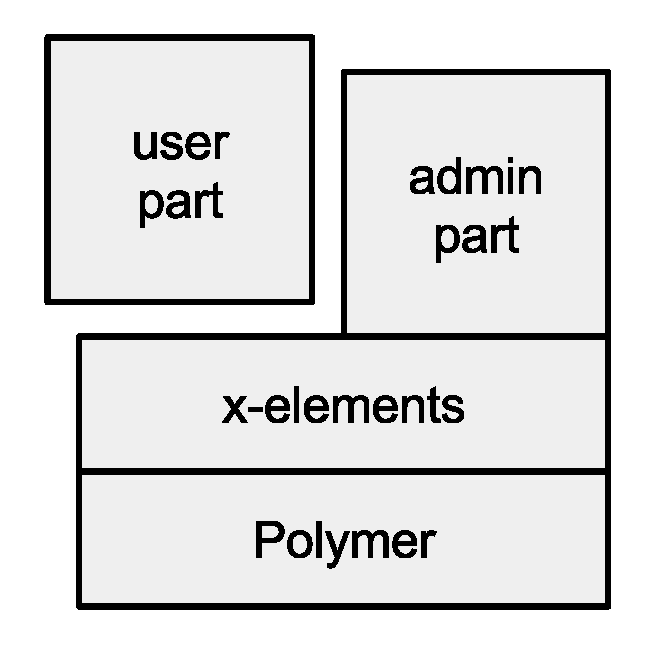
\epsfig{file=images/client-arch.eps, height=0.2\textwidth}
% \caption{Client-side architecture}
% \label{fig:client-arch}
% \end{figure}

